%---------------------------------------------------------------------
%
%                          Cap�tulo 4
%
%---------------------------------------------------------------------

\chapter{Design Study}

\begin{FraseCelebre}
\begin{Frase}
Surf it, scroll it, pause it, click it,\\
cross it, crack it, switch - update it\\
name it, rate it, tune it, print it,\\
scan it, send it, fax - rename it\\
Touch it, bring it, pay it, watch it.
\end{Frase}
\begin{Fuente}
Thomas \& Guy-Manuel, Daft Punk
\end{Fuente}
\end{FraseCelebre}

\begin{resumen}
In this chapter the platform design is described. Design decisions, specifications, schemes and needed calculations will be exposed.
Detailed characteristics of any chosen component, including microcontroller, radio interfaces, power-supply options will be provided.
\end{resumen}



%-------------------------------------------------------------------
\section{Global Hardware Description}
%-------------------------------------------------------------------
\label{cap4:sec:hardwareDescription}
%-------------------------------------------------------------------

Attending to the already described requirements and the conclusions obtained from the \ac{FCD} review, the following decisions have been taken before proceeding with the design process.

The whole system is thought as a teaser. Consisting on different fittable modules giving flexibility to the scheme. Main module, \ac{CNGD}, is the cornerstone. \ac{CNGD} supposes the main platform of the design, hosting the power supply system, possibilities to embed up to three \ac{RI}s, a control core unit, and other interfacing possibilities studied further on. As part of this modular design, the interfaces \ac{CNGD} hosts open possibilities to new extension board implementations through a pair of headers. These attachable boards, following the popular way these such of devices are called, will be referred as shields.  

Offering the chance of embedding up to three \ac{RI}s, the device could access three different frequency bands over the spectrum, fulfilling one of the desired requirements described in section \ref{cap3:sec:systemRequirements}. The chosen operation frequencies in our design are 434 MHz, 868 MHz, and 2.4 GHz, coupling the \ac{ISM} bands in most part of Europe. These bands are preferred for \ac{WSN} due to the data-rate, transmission power, and transmission range parameters they offer for a free cost. This configuration places the device on the bound of complexity and cost. At the same time, this feature is essential for a \ac{CWSN} proper investigation, giving radio communication opportunities not provided by any other similar device so far. Moreover, a full exploitation of the firmware described in \ref{cap3:sec:halreview} can be done, since it offers an integrated MiWi$^{TM}$ stack for three \ac{RI}s.

The three \ac{RI} are based on the IEEE 802.15.4 standard for \ac{WPAN}s, commonly used in \ac{WSN}. Specifically, the set of interfaces will operate under MiWi$^{TM}$ or MiWi$^{TM}$P2P protocol. They both are proprietary protocols designed by Microchip Technology that uses small, low-power digital radios. They are open source option designed for low data transmission rates (up to 250Kbit/s) and short distance (up to 100 without obstacles), cost constrained networks. Main difference between MiWi$^{TM}$ and ZigBee$^{TM}$\footnote{A very popular wireless IEEE 802.15.4 compatible protocol employed at \ac{WSN}s.} is complexity. MiWi$^{TM}$ offers a much more simple operation, resulting in a lighter implementation. The size required for the MiWi$^{TM}$ stack is  3-10 KB on the ROM depending on the node role while ZigBee$^{TM}$ takes 20-40 KB. MiWi$^{TM}$ is free of cost and it does not require for licenses acquisition as long as Microchip components are used, in fact Microchip requires the use of MiWi$^{TM}$ for its products. The global design becomes simpler and more homogeneous sharing a common communication protocol for all the \ac{RI}s.

Since there were not found compatible and suitable size commercial options for 434 MHz band, a custom full implementation of this interface was required. This implementation is based on MRF49XA transceiver, which can operate also at 868 MHz. In order to provide homogeneity, and since it does not suppose a great extra effort, the new \ac{RI} design will be used for both 434 and 868 MHz bands. These \ac{RI} will be called $\mu$Trans434/868 from now on. $\mu$Trans434/868 full description is taken at section \ref{cap4:sec:transceivers}. Option at 2.4 GHz is a MRF24J40MA module.

For this work a pair of shields were designed. A simple serial communication complement that links one \ac{UART} and a classic rs232 interface over the so-called rs232SHIELD. This interface would facilitate the software development since the firmware just allowed debugging through the \ac{UART} at first and it is described in section \ref{cap4:sec:rs232shield}. A battery charger Ni-Mh and Ni-Cd was also designed and implemented as a utility for portability options. The device was called as chargerSHIELD. 

Therefore, the set of designs to carry out, covered at Figure \ref{fig:cap4:globalhw}, includes $\mu$Trans 434 and 868, \ac{CNGD}, rs232SHIELD and chargerSHIELD.

\figura{Vectorial/Capitulo4/modules2develop}{width=.8\textwidth}{fig:cap4:globalhw}%
{Global hardware modules of the platform to develop.}

%-------------------------------------------------------------------
\section{Tools}
%-------------------------------------------------------------------
\label{cap4:sec:tools}
%-------------------------------------------------------------------


%-------------------------------------------------------------------
\subsection{Altium Designer}
%-------------------------------------------------------------------
\label{cap4:sub:altiumDesigner}
%-------------------------------------------------------------------

For the whole designing task, a \ac{EDA}\footnote{Electronic design automation is a category of software tools for designing electronic systems such as printed circuit boards and integrated circuits.} software will be use. Altium Designer, being one of the most important \ac{EDA} softwares, is commonly used by researchers at \ac{LSI}. All the \ac{CNGD} design process is carried through Altium Designer on its version 10. 

Altium Designer is software package for printed circuit board, \ac{FPGA} and embedded software design, and associated library and release management automation. It is developed and marketed by Altium Limited of Australia.

\figura{Bitmap/Capitulo4/altium}{width=.3\textwidth}{fig:cap4:altium}%
{Altium Designer logo}

Despite the amount of functions offered by Altium Designer the two main options needed for this project are schematic capture, for circuit edition, and \ac{PCB} design, for subsequent layout deployment.

Options provided by the schematic capture module, required for the design task, includes:

\begin{itemize}
	\item \emph{Component library management}. Useful to create own components facing the logic design.
	\item \emph{\ac{SPICE} mixed-signal circuit simulation}. In order to simulate any functionality. Specially useful in analog modules 			design.
      	\item \emph{Netlist export}. This way, it is possible to export our designs easily to process under other softwares.
     	\item \emph{Reporting and \ac{BoM} facilities}. For simple management purposes.
	\item \emph{Multi-channel, hierarchical schematics and design re-use}. Facilitating the design task.
\end{itemize}

On the other hand, required option from the \ac{PCB} design module are:
\begin{itemize}
	\item \emph{Component footprint library management}. Equally useful to manage new components and embed them into our \ac{PCB} designs.
   	\item \emph{Component placement}. In order to freely design our own layouts.
   	\item \emph{Manual trace routing, with support for multi-trace routing}. Enabling and facilitating the layout design.
   	\item \emph{Interactive 3D editing of the board and MCAD export to STEP}. To obtain more realistic views and complete idea of our 			implementations on advance to their manufacturing.
   	\item \emph{Manufacturing files generation with support for Gerber formats}. Essential for manufacturing process.
\end{itemize}

%-------------------------------------------------------------------
\section{Components Library: cngd lib}
%-------------------------------------------------------------------
\label{cap4:sec:cngdlib}
%-------------------------------------------------------------------
For the accomplish the full design of the platform over Altium Designer, a component library with all the required but not found models was set all along the design process.

As said, the library includes models from all those components needed but not found as well as modifications of existing models in order to suit the design criteria. Every contained model embeds schematic, footprint and 3D model. 3D models are useful for 3D rendering and proper hardware fitting checking purposes. Electric models of components are not generally included.

Library is available for download at ************************. All the content included into the library is ready to be used under Altium Designed. Any use of the library is free. 

\begin{figure}[h]
\centering

\subfloat[cNGD logo footprint.]{\label{fig:cap4:cognitivefoot}
\includegraphics[width=0.4\textwidth]{Imagenes/Vectorial/Capitulo4/cngdfoot}}%
\qquad
\subfloat[LSI logo footprint.]{\label{fig:cap4:lsifoot}
\includegraphics[width=0.2\textwidth]{Imagenes/Vectorial/Capitulo4/lsifoot}}%

\caption{Footprints specially designed for the platform.}
\label{fig:cap5:footprints}

\end{figure}


%-------------------------------------------------------------------
\section{Transceivers - $\mu$Trans 434/868}
%-------------------------------------------------------------------
\label{cap4:sec:transceivers}
%-------------------------------------------------------------------

\figura{Vectorial/Capitulo4/mtrans2develop}{width=.7\textwidth}{fig:cap4:mtranshw}
{$\mu$Trans detail over global hardware modules to develop.}

The chosen firmware for our platform gives support for MRF49XA modules over 434 MHz and 868 MHz bands. Specifically, the modules used during the firmware development were the MRF49XA PICtail$^{TM}$ Daughter Board\cite{daughterb}. This board is a demonstration and development daughter board for the MRF49XA ISM Band Sub-GHz RF Transceiver. The board can plug into a fittable header, which makes it unsuitable for a reduced size and robust \ac{WSN} design. It either accepts connection to external antennas, which is a desirable requirement.

Previous to the \ac{CNGD} designing, which will embeds the $\mu$Trans 434/868, the design of these \ac{RI}s was needed.

\figura{Bitmap/Capitulo4/mtransblocks}{width=.8\textwidth}{fig:cap4:mtransblocks}%
{$\mu$Trans 434/868 blocks diagram}

%-------------------------------------------------------------------
\subsection{Description}
%-------------------------------------------------------------------
MRF49XA is a low-power fully integrated Sub-GHz RF transceiver. An ideal choice for low-cost, high-volume, low data rate (< 256 Kbps), two-way, short range wireless applications. It can operate in the unlicensed 434, 868 and 915 MHz frequency bands. The transceiver is integrated with different sleep modes and an internal wake-up timer to reduce the overall current consumption. The device operates in the low-voltage range of 2.2V to 3.8V, and in Sleep mode, it operates at a very low-current state, typically 0.3 $\mu$A.

Further details are given below:
\begin{itemize}
	\item Modulation Technique: \ac{FSK} with \ac{FHSS} capability. 
	\item Differential RF Input/Output:
	\begin{itemize}
		\item -110 dBm Typical sensitivity with 0 dBm maximum input level.
		\item +7 dBm Typical transmit output power.
	\end{itemize}
	\item Maximum supported data rates:
	\begin{itemize}
		\item Digital mode 115.2 Kbps.
		\item Analog mode 256 Kbps.
	\end{itemize}
	\item Current Consumption:
	\begin{itemize}
		\item TX. 434MHz, I = 23 mA at 7 dBm. 868MHz, I = 24 mA at 5 dBm.
		\item RX. 433MHz, I = 11 mA. 868MHz, I = 12 mA.
		\item Idle. 1.2 mA (Max).
	\end{itemize}	
	\item Temperature range of operation from -40$^{\circ}$	to 85$^{\circ}$.
	\item Other functionalities: \ac{DQI} data, \ac{RSSI} data.
\end{itemize}

This transceiver is not IEEE 802.15.4 compatible since the number of channels it provides depends on the configured bit-rate, whereas the standard sets a fix number of channels. MRF49XA supports Microchip proprietary sub-GHz wireless protocols. 

Due to the \ac{RSSI} and \ac{DQI} indicators, the transceiver is able to carry out \ac{ED} scans over the supported frequencies to operate
on the least-noisy channel. This sensing capability is crucial for \ac{CR} tasks.

\figura{Bitmap/Capitulo4/mrf49xapinout}{width=.6\textwidth}{fig:cap4:mrf49xapinout}%
{MRF49XA pin diagram}

Figure \ref{fig:cap4:mrf49xapinout} shows the MRF49XA pin diagram, a full description of each pin is given here: 

\begin{itemize}
	\item 1. \emph{SDI}. Digital Input. Serial data input interface to MRF49XA (\ac{SPI} input signal).
	\item 2. \emph{SCK}. Digital Input. Serial clock interface (\ac{SPI} clock).
	\item 3. \emph{nCS}. Digital Input. Serial interface chip select (\ac{SPI} chip/device select).
	\item 4. \emph{SDO}. Digital Output. Serial data output interface from MRF49XA (\ac{SPI} output signal).
	\item 5. \emph{IRO}. Digital Output. Interrupt Request Output: Receiver generates an active-low interrupt request for the 					microcontroller on the terminated events. Some of this events are:
		\begin{itemize}
		\item Data-flow control registers notifications. 
		\item Negative pulse on interrupt input pin.
		\item Wake-up timer time-out.
		\item Supply voltage below the programmed value is detected.
		\item Power-on Reset.
		\end{itemize}

	\item 6. \emph{FSEL}. Digital Input/Output. \ac{FIFO} Select: Selects the FIFO and the first bit appears on the next clock when reading 						the Receiver FIFO Read Register. The FSEL pin has an internal pull-up resistor. This pin must be 						``high'' when the TX register is enabled. In order to achieve minimum current consumption, keep this pin 						``high'' in Sleep mode. This pin could provide other functionalities not used for our design.
	\item 7. \emph{FINT}. Digital Input/Output. \ac{FIFO} Interrupt: When the FIFO enable bit of General Configuration Register is 			enabled, this pin acts as a FIFO full interrupt, indicating that the FIFO has be en filled to its programmed limit. This pin 		could provide other functionalities not used for our design.
	\item 8. \emph{CLKOUT}. Digital Output. Clock Output: The transceiver's clock output can be used by the host microcontroller as a clock 				source.
	\item 9. \emph{RFXTL}. Analog Input. RF Crystal: This pin is connected to a 10 MHz series crystal or to an external oscillator 				reference. The crystal is used as a reference for the \ac{PLL} which generates the local oscillator frequency. It is 				possible to ``pull'' the crystal to the accurate frequency by changing the load capacitor value.
	\item 10. \emph{nRESET}. Digital Input/Output. Active-low hardware pin. This pin has an open-drain Reset output with internal pull-up 					and input buffer.
	\item 11. \emph{Vss}. Ground. Ground reference.
	\item 12. \emph{RFP}. RF. Input/Output Differential RF input/output (+).
	\item 13. \emph{RFN}. RF. Input/Output Differential RF input/output (-).
	\item 14. \emph{VDD}. Power. RF power supply. Bypass with a capacitor close to the pin. 
	\item 15. \emph{RSSIO}. Analog Input/Output. Received Signal Strength. Indicator Output: The analog RSSI output is used to determine the 					signal strength. The response and settling time depends on the external filter capacitor.
	\item 16. \emph{nINT}. Digital Input/Output. Interrupt: This pin can be configured as an active-low external interrupt to the device. 			If a logic '0' is applied to this pin, it causes the IRO pin to toggle, signaling an interrupt to the external microcontroller. 		The source of interrupt can be determined by reading the first four bits of STSREG. This pin can be used to wake-up the device 			from Sleep. This pin could provide other functionalities not used for our design.
\end{itemize}

An internal transmit/receive switch combines the transmitter and receiver circuits into differential RFP and RFN pins. These pins are connected to the impedance matching circuitry (balun) and to the external antenna connected to the device.

The quality of the data is checked or validated using the RSSI and DQI blocks built into the transceiver. Data is buffered in transmitter registers and receiver \ac{FIFO}s. The Automatic Frequency Control feature allows the use of a low-accuracy and low-cost crystal. The transceiver is controlled via a 4-wire SPI, interrupt (INT and IRO), FSEL, FINT and RESET pins. 

The complete design of the $\mu$Trans 434/868 is based on the implementation guidelines provided my Microchip at MRF49XA datasheet. The only difference between 434 MHz and 868 MHz version of the $\mu$Trans is the impedance matching circuitry facing the external antenna. The components composing it are different for each frequency band, values are specified at table \ref{tab:cap4:balunvalues} placed at appendix \ref{ap1:schematics}. 

Current is bypassed through a capacitor and supplies the MRF49XA, a power indication \ac{LED} is included in the design. A 10 MHz clock carries out the timing tasks. An impedance matching circuitry composed by inductors and capacitors interfaces the MRF49XA and the antenna. The \ac{RI} hosts a 50$\Omega$ connector to which connect the corresponding antenna.

The designed module allow access to some of the MRF49XA pins, not all of them. The ports accessible at the \ac{RI} are Interrupt (nINT), Interrupt Request Output, \ac{SPI} ports, \ac{FIFO} select, \ac{FIFO} interrupt, and reset. These ports enable full functionality of the MRF49XA and rest of available pins are found dispensable.

\figura{Bitmap/Capitulo4/mtransmodel}{width=.4\textwidth}{fig:cap4:mtransmodel}%
{$\mu$Trans 434/868 component model for use}

%-------------------------------------------------------------------
\subsection{Schematics}
%-------------------------------------------------------------------

Schematic of $\mu$Trans 434/868 can be found on Appendix \ref{ap1:schematics} at Figure \ref{ap1:mtransschematic}. Table \ref{tab:cap4:balunvalues} contains the different values for the balun circuit at 434 MHz and 868 MHz.  

%-------------------------------------------------------------------
\section{Main Board - cognitiveNextGenerationDevice}
%-------------------------------------------------------------------
\label{cap4:sec:cNGD}
%-------------------------------------------------------------------
\figura{Vectorial/Capitulo4/cngd2develop}{width=.4\textwidth}{fig:cap4:cngdhw}
{cNGD detail over global hardware modules to develop.}

%-------------------------------------------------------------------
\subsection{Description}
%-------------------------------------------------------------------
As it was said, \ac{CNGD} supposes the main part of the design, it hosts main capabilities for computation, power supply, and connectivity for the platform. It has being designed seeking simplicity and functionality.

The computation unit is located at the microcontroller, taking control over the rest of modules and running the software. This microcontroller can be programmed through its PGE port thanks to a PGE module that interfaces it.  

As part of the main goal, the firmware reviewed in section \ref{cap3:sec:halreview} will be used. It supposes an approach to the requirements achievement since it gives support for three interfaces, it supposes a reduction on the computation load and therefore, on the needed resources and power consumption. Moreover it will facilitate the development, offering a stable firmware version to work over and avoiding software development tasks. This fact will force the design to keep one architecture compatible with the firmware, hence a 32-bit Microchip PIC is required as microcontroller.

Communication and control over the \ac{RI}s is made through \ac{SPI}s and a few more control signal described further on. 

Power supply will be able to take place through three ways, a $\mu$USB, a block terminal and a DC terminal. Two first options will take a 5V supply, whereas the third one will take 3.3V. This last option is thought to be supplied by a battery. $\mu$USB option serves as serial communication chance, and since \ac{USB} provides 5V power supply, this is employed. A second 5V supplying connector opens possibilities to not compulsory use\ac{USB}. A software-driven power supply system to the \ac{RI}s allows the application to control the power supply to these modules. 

The device offers serial communication through the already named $\mu$USB options. Moreover, it gives access to to different peripherals through a pair of 20-pin headers. The list of approachable peripherals and pins covers battery connection (for charging purposes), \ac{GPIO}s, \ac{MCLR} pin, external interruptions, analogue inputs, \ac{USB}, Ethernet module, I2C bus, \ac{UART}s and \ac{SPI}. These option gives flexibility, modularity and versatility to the device. It provides possibilities for multiple kind of applications and open the design to new implementations and extensions for a particular applications. In addition, three \ac{LED}s and two push buttons give chance to the user to control the application if required. 

\figura{Vectorial/Capitulo4/cngdblocks}{width=.8\textwidth}{fig:cap4:modelcngd}%
{Architecture model of the cNGD.}
%-------------------------------------------------------------------
\subsection{Schematics}
%-------------------------------------------------------------------

Schematics can be found all together on Appendix \ref{ap1:schematics} for better convenience. Figure \ref{fig:cap4:gneralschematic} gathers all the modules into one global scheme. Figure \ref{fig:cap4:mcuschematics} shows the \ac{MCU} connections schematic. Figures \ref{fig:cap4:434schematics}, \ref{fig:cap4:868schematics}, and \ref{fig:cap4:2.4schematics} focus on 434MHz, 868MHz and 2.4GHz \ac{RI}s, respectively. Figure \ref{fig:cap4:powersupplyschematic} gives the schematic of the power supply system. Expansion headers schematic is on Figure \ref{fig:cap4:headerschematic}, whereas Figure \ref{fig:cap4:oscillatorschematic}, and \ref{fig:cap4:pgeschematic} illustrate the oscillator and programmer modules.

%-------------------------------------------------------------------
\subsection{Microcontroller}
%-------------------------------------------------------------------
Core unit is a PIC32MX675F256L\cite{pic32datasheet}, a mid-range 100-pin microcontroller from the mentioned 32-bit PIC family. Being the simplest of the options meeting memory performance and peripherals minimum requirements (Table \ref{cap3:tab:micros}). On the other hand, its 100 pins allow a better access of the peripherals provided. A larger memory version of this, PIC32MX675F512L, is pin compatible to the firstly mentioned. This fact gives the chance to swap among these two \ac{MCU}s if larger memory was needed. Main technical features follow:

\begin{itemize}
	\item Operating Voltage Range: 2.3V to 3.6V.
	\item 256/512 KB Flash (PIC32MX675F256L/PIC32MX675F512L). 64KB RAM.
	\item RUN, IDLE, and SLEEP modes. Multiple switchable clock modes for each power mode. Maximum speed is 80 MHz.
	\item Serial Communication Modules allow flexible UART/SPI/I2C configuration. 6 \ac{UART}s, 4 \ac{SPI}s, and 5 {I2C}s included.  
	\item USB 2.0 On-The-Go peripheral with integrated PHY.
	\item 10/100 Ethernet MAC with \ac{MII}/\ac{RMII}\footnote{Media Independent Interface and Reduced Media Independent Interface are standard 			interfaces used to connect a Fast Ethernet \ac{MAC}-block to a PHY chip.} interfaces. 
	\item 2 wire programming and debugging interface.
	\item Five 16-bit Digital Timers embedded.
	\item 16 channel 10-bit \ac{ADC}. 
\end{itemize}

Figure \ref{fig:cap4:pic32blocks} shows a block diagram of the PIC32 family. Distinct 32-bit buses for peripherals and system can be observed. Moreover, \ac{DMA}, \ac{RAM}, and flash controllers, together with external modules take place on it.

\figura{Bitmap/Capitulo4/pic32blocks}{width=0.8\textwidth}{fig:cap4:pic32blocks}%
{PIC32 family block diagram}

The whole microcontroller can be divided into for blocks: core, memory, integration system and peripherals:

\begin{itemize}
	\item The main core is based on a \ac{RISC} MIPS M4K. This module takes control over the system. It controls the peripherals and execute 			the programmed code.

	\item A further observation into the memory system allows differentiate among Flash, \ac{RAM}, registers, and boot flash. The system 			load the data on a cache memory and prefetch the instructions. Figure \ref{fig:cap4:pic32cachemodule} shows the block diagram of the prefetch module.

\figura{Bitmap/Capitulo4/cache}{width=0.7\textwidth}{fig:cap4:pic32cachemodule}%
{Prefetch cache module block diagram.}	

	\item Integration system is compound by the set of modules needed to make work the core and peripherals. These are interrupt control, 			oscillator system, reset, watchdog timer and power-up timer. For detailed explanation of each module consult the microcontroller 			manual \cite{pic32datasheet}.

	\item Peripherals are a set of independent modules oriented to perform specific tasks. Here it is described a brief description of the 			main peripherals and the use they receive in the system: 

	\begin{itemize}
		\item \emph{\ac{SPI}}. The SPI module is a synchronous serial interface that is useful for communicating with external 					peripherals and other microcontroller devices. These peripheral devices may be serial \ac{EEPROM}, shift 					registers, display drivers, etc. 

				At \ac{CNGD}, three \ac{SPI}s are used to set communication with the \ac{RI}s. Another \ac{SPI} is outputted to 					the expansion headers for general purposes.

				
		\item \emph{\ac{UART}}. This peripheral is a serial I/O module. The \ac{UART} is a full-duplex, asynchronous communication
				 channel that communicates with peripheral devices and personal computers through protocols, such as RS-232, 					RS-485, LIN 1.2 and \ac{IRDA}.

				Two \ac{UART} modules are available at the expansion headers. RS232Shield described at section \ref{cap4:sec:rs232shield} use one of this modules to set an RS-232 serial interface.

		\item \emph{\ac{USB} \ac{OTG}}. The \ac{USB} module contains analog and digital components to provide a \ac{USB} 2.0
			full-speed and low-speed embedded Host, full-speed Device or \ac{OTG} implementation with a minimum of external 			components. 				
			
			This \ac{USB} peripheral is used to establish serial communication with other devices, \ac{CNGD} it thought to include 				this serial communication way. Its ease of use, popularity, makes it a good choice for this purpose. Moreover, it is 				interfaced into the expansion headers for other future uses.
	
		\item \emph{\ac{I2C}}. The \ac{I2C} module provides complete hardware support for both Slave and Multi-Master modes of the \ac{I2C} serial communication standard. 
			This module is commonly used to establish communication among sensors and microcontroller. One \ac{I2C} can be accessed 			over the expansion headers.

		\item \emph{TIMERS}. Four synchronous, one asynchronous, 16-bit timers that can operate as a free-running interval timer for 				various timing applications and counting external events.

			This timers, properly configured, will drive in time the firmware operation. This includes, pretty much, all the tasks 				carried out by the node. Timers also must be available to drive in time the application if was required. 

		\item \emph{\ac{ADC}}. It converts a continuous voltage quantity to a digital number that represents the quantity's amplitude. 

			Useful when dealing with sensors offering an analog output signal. The \ac{ADC} included into the microcontroller can be 				accessed from the expansion headers.

		\item \emph{ETHERNET}. The Ethernet controller is a bus master module that interfaces with an off-chip Physical Layer (PHY) to
			implement a complete Ethernet node in a system.
			
			This module is accessible at the headers. It is essential to establish 802.11 communications, which is a desirable 				feature for \ac{WSN} coordinator nodes or gateways.

		\item \emph{\ac{GPIO}}. General purpose I/O pins are the simplest of peripherals. They allow the PIC32 MCU to monitor and control
			other devices. Basically, almost every pin at the \ac{MCU} can act as a \ac{GPIO} if no other peripherals are active and 				multiplexed on such pin.

			Several \ac{GPIO}s can be accessed over the headers for general purposes.

		\item \emph{\ac{RTCC}}. It is intended for applications in which accurate time must be maintained for extended periods of time
			with minimal or no CPU intervention. Low-power optimization provides extended battery lifetime while keeping track of 				time.

			This module is essential for accurate timing tasks, which are common in \ac{WSN} for synchronous processes over the 				network. Synchronization helps saving energy since it allows better efficient communication and general operation.
	\end{itemize}  
\end{itemize}

%-------------------------------------------------------------------
\subsubsection{Pin-out}
%-------------------------------------------------------------------
Here is described the multiplexed functionalities available on each pin at the \ac{MCU}. Functionalities emphasized in bold are functionalities available for use, not emphasized functionalities are not usable with the current design. In addition, module where the pin is used and linked signal are exposed. For further details about peripherals and pins description see the PIC32 family reference manual\cite{pic32datasheet}.  

{\footnotesize
\begin{longtable}{l l l l l}
% aqu� a�adimos el encabezado de la primera hoja.
\hline
PIN & PERIPHERALS &  MODULE & USE \\
\hline \hline
\endfirsthead

% aqu� a�adimos el encabezado del resto de hojas.
\hline
PIN & PERIPHERALS & MODULE & USE \\
\hline \hline
\endhead

% aqu� a�adimos el fondo de todas las hojas, excepto de la �ltima.
\multicolumn{4}{c}{Follows on next page.}
\endfoot

% aqu� a�adimos el fondo de la �ltima hoja.
\endlastfoot

% aqu� a�adimos el cuerpo de la tabla.
1 & AERXARR/RG15 & - & -  \\ \hline
2 & VDD & \multicolumn{2}{l}{Power Supply} \\ \hline
3 & PMD5/\textbf{RE5} & Header & p23 \\ \hline
4 & PMD6/\textbf{RE6}  & Header & p35 \\ \hline
5 & PMD7/\textbf{RE7}  & Header & p22 \\ \hline
6 & T2CK/\textbf{RC1}  & Header & p36\\ \hline
7 & T3CK/RC2 &  - & - \\ \hline
8 & T4CK/RC3 &  - & -  \\ \hline
9 & T5CK/\textbf{SDI1}/RC4 & \ac{RI} 434MHz & SPI SDO\\ \hline
10 & ECOL/\textbf{SCK2}/\textbf{U6TX}/\textbf{U3nRTS}/PMA5/\textbf{CN8}/\textbf{RG6} & Header & p37  \\ \hline
11 & ECRS/\textbf{SDA4}/\textbf{SDI2}/\textbf{U3RX}/PMA4/\textbf{CN9}/\textbf{RG7} & Header & p21  \\ \hline
12 & \textbf{ECRSDV}/\textbf{SCL4}/\textbf{SDO2}/\textbf{U3TX}/PMA3/\textbf{CN10}/\textbf{RG8} & Header & p38  \\ \hline
13 & \textbf{nMCLR} & PGE/Pushbutton & Reset \\ \hline
14 & \textbf{EREFCLK}/nSS2A/\textbf{U3nCTS}/\textbf{U6RX}/PMA2/\textbf{CN11}/\textbf{RG9} & Header & p20 \\ \hline
15 & VSS &  \multicolumn{2}{l}{Ground} \\ \hline
16 & VDD &  \multicolumn{2}{l}{Power Supply} \\ \hline
17 & TMS/RA0 & - & -  \\ \hline
18 & AERXD0/\textbf{INT1}/RE8 & \ac{RI} 434MHz & Interrup. \\ \hline
19 & AERXD1/\textbf{INT2}/\textbf{RE9} & Header & p00 \\ \hline
20 & \textbf{AN5}/\textbf{C1IN+}/\textbf{VBUSON}/\textbf{CN7}/\textbf{RB5} & Header & p01 \\ \hline
21 & \textbf{AN4}/\textbf{C1IN-}/\textbf{CN6}/\textbf{RB4} & Header & p39 \\ \hline
22 & \textbf{AN3}/C2IN+/\textbf{CN4}/\textbf{RB3} & Header & p02 \\ \hline
23 & AN2/C2IN-/CN3/RB2 & - & - \\ \hline
24 & \textbf{PGEC1}/AN1/CN2/RB1 & PGE & PGEC \\ \hline
25 & \textbf{PGED1}/AN0/CN1/RB0 & PGE & PGED \\ \hline
26 & PGEC2/AN6/OCFA/RB6 & - & - \\ \hline
27 & PGED2/AN7/\textbf{RB7} & \ac{RI} 434MHz & Reset \\ \hline
28 & \textbf{VREF-}/\textbf{CVREF-}/AERXD2/PMA7/\textbf{RA9} & Header & p18\\ \hline
29 & \textbf{VREF+}/\textbf{CVREF+}/AERXD3/PMA6/\textbf{RA10} & Header & p19  \\ \hline
30 & AVDD & \multicolumn{2}{l}{Power Supply} \\ \hline
31 & AVSS & \multicolumn{2}{l}{Ground} \\ \hline
32 & AN8/C1OUT/\textbf{RB8} & \ac{RI} 434MHz & Wake \\ \hline
33 & AN9/C2OUT/\textbf{RB9} & \ac{RI} 434MHz & Power Switch \\ \hline
34 & AN10/CVREFOUT/PMA13/\textbf{RB10} & \ac{RI} 434MHz & Chip Select \\ \hline
35 & \textbf{AN11}/\textbf{ERXERR}/AETXERR/PMA12/\textbf{RB11} & Header & p03 \\ \hline
36 & VSS &  \multicolumn{2}{l}{Ground}  \\ \hline
37 & VDD &  \multicolumn{2}{l}{Power Supply}\\ \hline
38 & TCK/RA1 & - & - \\ \hline
39 & \textbf{SCK4}/U5TX/U2nRTS/RF13 & \ac{RI} 2.4GHz & SPI SCK\\ \hline
40 & nSS34/U5RX/U2nCTS/\textbf{RF12} & \ac{RI} 868MHz & FIFO Int.\\ \hline
41 & \textbf{AN12}/\textbf{ERXD0}/AECRS/PMA11/\textbf{RB12} & Header & p04\\ \hline
42 & \textbf{AN13}/\textbf{ERXD1}/AECOL/PMA10/\textbf{RB13} & Header & p05 \\ \hline
43 & \textbf{AN14}/ERXD2/AETXD3/PMALH/PMA1/\textbf{RB14} & Header & p17\\ \hline
44 & \textbf{AN15}/ERXD3/OCFB/PMALL/PMA0/\textbf{CN12}/\textbf{RB15} & Header & p16\\ \hline
45 & VSS & \multicolumn{2}{l}{Power Supply}\\ \hline
46 & VDD & \multicolumn{2}{l}{Power Supply}\\ \hline
47 & AETXD0/nSS3/U4RX/U1nCTS/CN20/\textbf{RD14} & \ac{RI} 868MHz & FIFO Sel.\\ \hline
48 & AETXD1/\textbf{SCK3}/U4TX/U1nRTS/CN21/RD15 & \ac{RI} 868MHz  & SPI SCK\\ \hline
49 & SDA5/\textbf{SDI4}/U2RX/PMA9/CN17/RF4 & \ac{RI} 2.4GHz & SPI SDO \\ \hline
50 & SCL5/\textbf{SDO4}/U2TX/PMA8/CN18/RF5 & \ac{RI} 2.4GHz & SPI SDI\\ \hline
51 & \textbf{USBID}/\textbf{RF3} & USB/Header & USB ID/p06 \\ \hline
52 & SDA3/\textbf{SDI3}/U1RX/RF2 & \ac{RI} 868MHz & SPI SDO \\ \hline
53 & SCL3/\textbf{SDO3}/U1TX/RF8 & \ac{RI} 868MHz & SPI SDI \\ \hline
54 & \textbf{VBUS} & USB/Header & VBUS/p07 \\ \hline
55 & VUSB & \multicolumn{2}{l}{Power Supply + Cap} \\ \hline
56 & \textbf{D-}/\textbf{RG3} & USB/Header & D-/p13 \\ \hline
57 & \textbf{D+}/\textbf{RG2} & USB/Header & D+/p12 \\ \hline
58 & \textbf{SCL2}/\textbf{RA2} & Header & p11 \\ \hline
59 & \textbf{SDA2}/\textbf{RA3} & Header & p10 \\ \hline
60 & TDI/\textbf{RA4} & LEDS & LED 3 \\ \hline
61 & TDO/\textbf{RA5} & LEDS & LED 2\\ \hline
62 & VDD &  \multicolumn{2}{l}{Power Supply} \\ \hline
63 & \textbf{OSC1}/CLKI/RC12 & Oscillators & Prim. Osc. In. \\ \hline
64 & \textbf{OSC2}/CLKO/RC15 & Oscillators & Prim. Osc. Out. \\ \hline
65 & VSS &  \multicolumn{2}{l}{Ground}  \\ \hline
66 & AETXCLK/SCL1/\textbf{INT3}/RA14 & \ac{RI} 868MHz & Interrup. \\ \hline
67 & AETXEN/SDA1/\textbf{INT4}/RA15 & \ac{RI} 2.4GHz & Interrup. \\ \hline
68 & RTCC/\textbf{EMDIO}/AEMDIO/\textbf{IC1}/\textbf{RD8} & Header & p09 \\ \hline
69 & nSS1/\textbf{IC2}/\textbf{RD9} & Header & p32 \\ \hline
70 & \textbf{SCK1}/IC3/PMCS2/PMA15/RD10 & \ac{RI} 434MHz & SPI SCK\\ \hline
71 & \textbf{EMDC}/AEMDC/\textbf{IC4}/PMCS1/PMA14/\textbf{RD11} & Header & p27 \\ \hline
72 & \textbf{SDO1}/OC1/INT0/RD0 & \ac{RI} 434MHz & SPI SDI \\ \hline
73 & \textbf{SOSCI}/CN1/RC13  & Oscillators & Sec. Osc. In.\\ \hline
74 & \textbf{SOSCO}/T1CK/CN0/RC14 & Oscillators & Sec. Osc. Out.\\ \hline
75 & VSS &  \multicolumn{2}{l}{Ground}  \\ \hline
76 & OC2/\textbf{RD1} & \ac{RI} 868MHz & Reset\\ \hline
77 & OC3/\textbf{RD2} & \ac{RI} 868MHz & Wake\\ \hline
78 & OC4/\textbf{RD3} & \ac{RI} 868MHz & Power Switch\\ \hline
79 & ETXD2/IC5/PMD12/RD12 & - & - \\ \hline
80 & ETXD3/PMD13/CN19/RD13 & - & - \\ \hline
81 & OC5/PMWR/CN13/\textbf{RD4} & \ac{RI} 868MHz & Chip Select \\ \hline
82 & PMRD/\textbf{CN14}/\textbf{RD5} & Push buttons & S2 \\ \hline
83 & \textbf{ETXEN}/PMD14/\textbf{CN15}/\textbf{RD6} & Header & p33\\ \hline
84 & ETXCLK/PMD15/\textbf{CN16}/\textbf{RD7} & Push buttons & S3\\ \hline
85 & VCAP/VDDCORE & \multicolumn{2}{l}{Capacitor} \\ \hline
86 & VDD &  \multicolumn{2}{l}{Power Supply} \\ \hline
87 & \textbf{ETXD1}/PMD11/\textbf{RF0} & Header & p26\\ \hline
88 & \textbf{ETXD0}/PMD10/\textbf{RF1} & Header & p25\\ \hline
89 & ETXERR/PMD9/RG1 & - & - \\ \hline
90 & PMD8/RG0 & - & - \\ \hline
91 & TRCLK/\textbf{RA6} & LEDS & LED1 \\ \hline
92 & TRD3/RA7 & - & - \\ \hline
93 & PMD0/\textbf{RE0} & \ac{RI} 2.4GHz & Reset\\ \hline
94 & PMD1/\textbf{RE1} & \ac{RI} 2.4GHz & Wake\\ \hline
95 & TRD2/\textbf{RG14} & \ac{RI} 434MHz & FIFO Sel.\\ \hline
96 & TRD1/RG12 & - & - \\ \hline
97 & TRD0/\textbf{RG13} & \ac{RI} 434MHz & FIFO Int. \\ \hline
98 & PMD2/\textbf{RE2} & \ac{RI} 2.4GHz & Power Switch\\ \hline
99 & PMD3/\textbf{RE3} & \ac{RI} 2.4GHz & Chip Select\\ \hline
100 & PMD4/RE4 & - & - \\ \hline
\\ % esta l�nea es importante para que deje un espacio entre la tabla y el nombre de la tabla.

\caption{PIC32675F256L pins use description.}
\label{tab:cap4:micropinout}

\end{longtable}}

%-------------------------------------------------------------------
\subsection{Radio Interfaces}
%-------------------------------------------------------------------
As it was mentioned, \ac{CNGD} will be able to include up to three \ac{RI}s, with three consequent frequency bands to access. This fact gives a flexibility over radio communications never offered by other \ac{WSN} device. Frequencies to operate over are 434 MHz, 868 MHz, and 2.4 GHz, meeting desired features. 

For communication on 434 MHz and 868 MHz, ad-hoc designed \ac{RI}s described in Section \ref{cap4:sec:transceivers} are used. These \ac{RI}s are based on the MRFX49XA radio transceiver and a full description of them can be found at such section. These \ac{RI}s share common features since the radio transceiver module is identical for both. This brings simplicity to the system. Interface between these \ac{RI}s and \ac{MCU}, illustrated at Figure \ref{fig:cap4:mrf49xainterface}, are the same. 

\figura{Bitmap/Capitulo4/mrf49xainterface}{width=0.5\textwidth}{fig:cap4:mrf49xainterface}%
{Microcontroller to MRF49XA interface}

Figure \ref{fig:cap4:2.4schematics} shows the scheme for the \ac{RI} at 2.4 GHz. This is based on a MRF24J40MA\cite{mrf24j40}. This \ac{RI} was already used at the \ac{FCD} and it is supported by the firmware. It is a MiWi$^{TM}$ transceiver also compatible with the IEEE 802.15.4 standard, this homogeneity with the other two \ac{RI}s supposes computation, cost, and power savings. It has access over the 15 5MHz-channels, the protocol enables and employs a \ac{QPSK} modulation. Figure \ref{fig:cap4:mrf24j40mablocks} shows the MRF24J40MA block diagram. Further details about the MRF24J40MA \ac{RI} follow:

\figura{Bitmap/Capitulo4/mrf24j40mablocks}{width=0.8\textwidth}{fig:cap4:mrf24j40mablocks}%
{MRF24J40MA block diagram.}

\begin{itemize}
	\item Operating Voltage: 2.4-3.6V (3.3V typical).
	\item Up to 120 meters range.
	\item Differential RF Input/Output:
	\begin{itemize}
		\item -94 dBm Typical sensitivity with +5 dBm maximum input level.
		\item +0 dBm Typical output power.
	\end{itemize}
	\item Maximum supported data rates:
	\begin{itemize}
		\item 250 Kbps.
		\item Turbo mode enables up to 625 Kbps (not following the standard).
	\end{itemize}
	\item Current Consumption:
	\begin{itemize}
		\item TX. I = 23 mA (typical).
		\item RX. 19 mA (typical).
		\item Sleep. 2$\mu$A (typical).
	\end{itemize}	
	\item Integrated crystal, internal voltage regulator, matching circuitry, \ac{PCB} antenna, and \ac{RSSI} detector. 
\end{itemize}

Interface between MRF24J40MA \ac{RI} is driven by 7 signals, figure \ref{fig:cap4:mrf24j40mainterface} illustrates it. Serial communication is carried through a \ac{SPI}, containing 4 signals. Two interruption signals for both senses and a reset signal complete the whole set.

\figura{Bitmap/Capitulo4/mrf24j40mainterface}{width=0.5\textwidth}{fig:cap4:mrf24j40mainterface}%
{MRF24J40MA interface scheme}

All the described \ac{RI}s are based on transceivers supporting either MiWi$^{TM}$ Mesh or MiWi$^{TM}$ P2P protocols. Figure \ref{fig:cap4:miwiconf} shows how the protocol environment configuration.

\figura{Bitmap/Capitulo4/miwiconf}{width=0.8\textwidth}{fig:cap4:miwiconf}{MiWi$^{TM}$ protocol configuration scheme.}

A network using the MiWi$^{TM}$ protocol\cite{miwi} is capable of having a maximum of 1024 nodes on a network. Each coordinator is only capable of having 127 children, with a maximum of 8 coordinators in a network. Packets can travel a maximum of 4 hops in the network and 2 hops maximum from the PAN coordinator. 

The MiWi$^{TM}$ P2P protocol\cite{miwip2p} stack supports star and peer-to-peer wireless-network topologies, useful for simple, short-range, wireless node-to-node communication. Additionally, the stack provides sleeping-node, active-scan and energy-detect features while supporting the low-power requirements of battery-operated devices.

\begin{figure}[h]
\centering
   
\subfloat[Standard stack.]{\label{fig:cap4:normalmiwistack}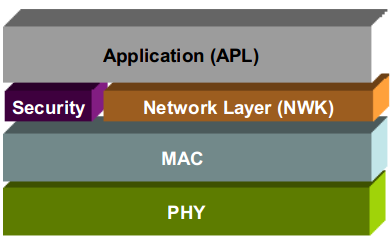
\includegraphics[width=.4\textwidth]{Imagenes/Bitmap/Capitulo4/miwistack}}  
\subfloat[Adapted stack for three RIs, available at the firmware.]{\label{fig:cap4:adaptedmiwistack}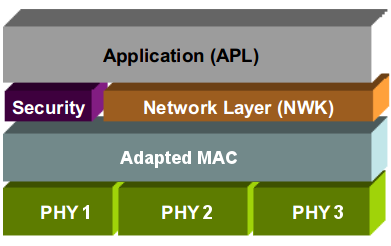
\includegraphics[width=.4\textwidth]{Imagenes/Bitmap/Capitulo4/adaptedmiwistack}}
       
\caption{MiWi$^{TM}$ Protocol.}
\label{fig:cap4:miwistack}
\end{figure}

%-------------------------------------------------------------------
\subsubsection{Software Controlled Power Supply}
%-------------------------------------------------------------------
The designed system allows enabling/disabling the power supply to the \ac{RI}s. This way, any \ac{RI} can be completely switched off by the running application. Cutting down all possible power consumption that unused \ac{RI}s could have by, for instance, running clocks.

The power control to the \ac{RI}s is based on the ADG701\cite{adg701}. This is a  \ac{CMOS} \ac{SPST} switch. This switch is designed to provide low power dissipation, low on resistance and low leakage currents. It can operate from a single 1.8 V to 5.5 V supply, making it ideal for use in battery-powered instruments.

Some of the features of this component are:
\begin{itemize}
	\item 2 ohm (typical) on resistance.
	\item Fast switching times: tON = 18 ns, tOFF 12 ns.
	\item Typical power consumption < 0.01 $\mu$W. 
\end{itemize}

\figura{Bitmap/Capitulo4/adg701}{width=.2\textwidth}{fig:cap4:adg701}%
{ADG701 pin diagram.}

Pin 4 (IN) is a digital input where the control logic signal is placed. A logic '1' will make pins 1 (D - drain) and  2 (S - source) shorted, a logic '0' will open the switch. Pins 1 and 2 can be either inputs or outputs. Pin 5 (NC) must not be connected.

In case ADG701 switch was not included into the design for any reason, optional 0 $\Omega$ resistors must be used to enable power supply at the \ac{RI}s. These optional resistors are R16, R17, and R18 for 434 MHz, 868 MHz, and 2.4 GHz \ac{RI}s respectively.  

%-------------------------------------------------------------------
\subsection{Power Supply System}
%-------------------------------------------------------------------
Power supply module is in charge of providing proper voltage and current to the \ac{CNGD}. Chosen output voltage is 3.3V, being this a normal value for \ac{CMOS} family chips. The power supply system must be able to support either wired-fixed or battery options. Figure \ref{fig:cap4:powersupplyschematic} shows a schematic of this module.

For external wired options, the input voltage is 5V. This value is widely used to supply digital circuits and it is easy to access to 5 V sources. Moreover, it couples with the \ac{USB} voltage rate, being possible to supply the \ac{CNGD} through a $\mu$USB terminal that this module includes. Apart from this \ac{USB} terminal, a standard screw terminal block accepts 5V to supply the device. This 5V are lowered to 3.3V by a synchronous buck regulator. This buck regulator can be deactivated for power saving when unused just changing a jumper location.

For battery options, the module includes a DC connector. This connector accepts from 3.3V up to 3.6V. Higher voltages could damage the components since this voltage is directly injected into the circuitry to achieve higher efficiency. An included switch lets choosing the supply mode, either wired or portable.

A green \ac{LED} indicates that power is applied into the circuit, on the other hand, a red \ac{LED} indicates if power is supplied into the block terminal or the $\mu$USB terminal. This way, is easily noticeable the presence of voltage and current on the \ac{CNGD} and their origin input.       

The employed synchronous buck regulator is a MCP1603\cite{mcp160} chip. This is a high-efficiency, fully-integrated 500 mA synchronous buck regulator with a 2.7V to 5.5V input voltage range. The MCP1603 is available with either an adjustable or fixed output voltage. The are several available fixed output voltage options, the chosen option here is 3.3V. When a fixed option is used, only three additional small external
components are needed to form a complete solution, Figure \ref{fig:cap4:mcp1603}.

\figura{Bitmap/Capitulo4/mcp1603}{width=0.5\textwidth}{fig:cap4:mcp1603}{MCP1603 buck regulator configuration.}

It was estimated that 500 mA was enough to supply the device regarding the described maximum consumptions. Table \ref{tab:cap4:maxconsumption} gives 165 mA as maximum current consumption rate. Leaving buffer for current peaks at transmission and possible shields, a maximum current estimation of 500 mA seem reasonable and enough for the whole platform.

\begin{table}[h]
\centering
\scalebox{0.9}{
\begin{tabular}{l r}
\hline
Module & Max. Power \\ \hline \hline
PIC32MX675F256L (Run mode) & 85 mA  \\ \hline
$\mu$Trans 434 (TX mode) & 23 mA \\ \hline
$\mu$Trans 868 (TX mode) & 24 mA \\ \hline
MRF24j40MA (TX mode) &  23 mA \\ \hline
LEDS  & 10 mA \\ \hline \hline
TOTAL MAX CONSUMPTION & 165mA \\ \hline 
\end{tabular}
}
\caption{Maximum estimated power consumption of the platform.
	\label{tab:cap4:maxconsumption}}
\end{table}

%-------------------------------------------------------------------
\subsubsection{Battery}
%-------------------------------------------------------------------
In order to give autonomy and portability to the device, a rechargeable battery system will be included. This system must keep down the global cost and size. At the same time it must offer autonomy to the device. Voltage offered by the battery system must be on the 3.3-3.6V range. 

Firstly it is needed an estimation of platform global current consumption. This value will depends, relying strongly on the running application. However, we can assume some overestimated common values for our study. Considering two operation modes, Run and Sleep, and using values of current and operation times at Table \ref{tab:cap4:powerstimatedvalues}, it results in an approximated global current consumption calculated as $C_{estimated}$.

\begin{table}[h]
\centering
\scalebox{0.9}{
\begin{tabular}{l r r}
\hline 
Mode & Operation time percentage & Consumption \\ \hline \hline
Run & 10\% & 120 mA \\ \hline
Sleep & 90\% & 100 $\mu$A \\ \hline
\end{tabular}
}
\caption{Estimated values for Run and Sleep operation modes.%
         \label{tab:cap4:powerstimatedvalues}}
\end{table} 

\[C_{estimated}= 100 \times10^{-3}  \times 0.1 + 100 \times10^{-6}  \times 0.90 = 12.1 ~ mA\]

Table \ref{tab:cap4:batcomparison} shows a comparison between considered battery possibilities. Other technologies and sizes, not described at the table, have been directly discarded for showing unsuitable features. An example are \ac{NICD} technology batteries, which may suffer ``memory effect''\footnote{It is an effect observed in some kind of rechargeable batteries that causes them to hold less charge.}, or special size batteries\footnote{For instance, 2/3 A, L-fat A, or CS sizes.} whose price is extremely high. Possible options considered are some \ac{NIMH}-based and \ac{LIION} based batteries. 

\begin{table}[h]
\centering
\scalebox{0.7}{
\begin{tabular}{||c|c|c|c|c|c|c|c||}
\hline
\hline
\multirow{2}{*}{Technology} & Cell Nominal & Min. Num. & \multirow{2}{*}{Use complexity} & \multirow{2}{*}{Size} & Capacity & Estimated & Aprox. \\ 
& Voltage & of cells  & & & (mHh) & autonomy (h.) & Unit. Cost (\euro)\\ \hline \hline
\multirow{2}{*}{Ni-MH} & \multirow{2}{*}{1.2/1.25 V} & \multirow{2}{*}{3} & \multirow{2}{*}{Low} & AAA & 600 - 1250 & 50 - 100 & 1 - 2  \\ \cline{5-8}
& & & & AA & 1200 - 2900 & 100 - 240 & 1.5 - 3 \\ \hline
\multirow{ 5}{*}{Li-ion} & \multirow{5}{*}{3.6/3.7 V} & \multirow{5}{*}{1} & \multirow{5}{*}{Medium} & AAA & 500 - 600 & 40 - 50 & 3.5 - 4.5 \\ \cline{5- 8}
 &  &  &  & AA & 900 &  75  & 4 - 6 \\ \cline{5- 8}
 &  &  &  & CR123A & 700 - 2000 & 60 - 165 & 3 - 20 \\ \cline{ 5- 8}
 &  &  &  & CR2 & 600 - 800 & 50 - 65  & 3.5 \\ \cline{ 5- 8}
 &  &  &  & Other & up to 3000 & up to 250  & 40 - 60 \\ \hline \hline
\end{tabular}}
\caption{Comparison among considered batteries.
\label{tab:cap4:batcomparison}}
\end{table}

Facing similar capacities, \ac{LIION} options show a higher cost than \ac{NIMH} even considering 3 \ac{NIMH} cells are needed. In addition, \ac{LIION} show difficulties for its use since \ac{LIION} batteries must include circuitry to control discharge cycles and other security issues. Charging process is more complex as well. 

The solution proposed consist of a battery consisting on 3 2900 mAh \ac{NIMH} AA cells. This might provide up to 240 h. of autonomy considering our estimations. No more circuitry is needed for the battery except for a 3-AA battery-holder. The total cost for a complete battery pack is under 10 \euro. 

%-------------------------------------------------------------------
\subsection{Timing}
%-------------------------------------------------------------------
The microcontroller includes possibilities to properly place quartz crystals in parallel with internal amplifiers and a pair of suitable capacitors in such way they work as oscillators. The oscillator signal is then connected to the internal \ac{PLL} to obtain the desired frequency. Figures \ref{fig:cap4:prioscillators} and \ref{fig:cap4:secoscillators} show the basic input scheme for primary and secondary oscillators respectively.

Primary oscillator is 8 MHz quartz crystal used as system reference clock. The respective \ac{PLL} is configured to raise this frequency up to 80 MHz. It exists the possibility of replacing the functionality of this clock for a internal one, but stability and accuracy can be affected.

\figura{Bitmap/Capitulo4/priosc}{width=.3\textwidth}{fig:cap4:prioscillators}%
{PIC32MX675F256L primary oscillator input.}

In order to calculate the values for $C_{1}$ and $C_{2}$ capacitors, we will use a common formula used for crystal-based oscillator design.

\[ 
C_{L} = \frac{C_{1}C_{2}}{C_{1}+C_{2}} + C_{P} + C_{I}
\]

Where $C_{1}$ and $C_{2}$ have an equal value, $C_{L}$ is the load capacitance required for the crystal, $C_{P}$ is the circuit parasitic capacitance and $C_{I}$ is the chip input capacitance. Typically $C_{P} + C_{I}$ is set to 5 pF. For the 8 MHz crystal, load capacitance specified by the manufacturer is 20 pF\cite{8mdatasheet}. The resulting equation remains like follows:

\[ 
20~ pF = \frac{C_{1}C_{2}}{C_{1}+C_{2}} + 5 ~ pF
\]

Resolving the equation, it results that $ C_{1} = C_{2} = 15 \quad pF$.
\\
Second oscillator, a 32.728 KHz, supposes a low-power clock for real time clocking. It enables nodes synchronization, which is fundamental for power-saving modes.

\figura{Bitmap/Capitulo4/secoscillator}{width=.4\textwidth}{fig:cap4:secoscillators}%
{PIC32MX675F256L second oscillator input.}

For this second clock, load capacitance comes to be 12.5 pF\cite{32kdatasheet}. Hence the corresponding equation results as follows:

\[ 
12.5~ pF = \frac{C_{1}C_{2}}{C_{1}+C_{2}} + 5 ~ pF
\]

Resulting capacitors value are $ C_{1} = C_{2} = 15 \quad pF$

%-------------------------------------------------------------------
\subsection{Expansion Headers}
%-------------------------------------------------------------------

Figure \ref{fig:cap4:headerschematic} shows the schematic design for this module. Basically, two headers, containing 20 pins each, enable access to unused and useful peripherals the microcontroller includes. This offers possibilities to future implementations and expansions for the node by simply attaching a device through these headers and carrying through the corresponding firmware adaptations. Possible attachable implementations are 802.11 interfaces, data acquisition modules, external memories, extra \ac{RI}s, etc.

Here it is made a comprehensive description of the available peripherals and functionalities at the headers:

\begin{itemize}
	\item \emph{Power Supply}. Several pins offer power supply options:
		\begin{itemize}
		\item VCC. Shorted to the \ac{CNGD} supply system available at the platform, usually 3.3V. Pins 14, 24, and 28.
		\item GND. Shorted to \ac{CNGD} ground. Pins 15, 31, and 34.	
		\item BAT+. Directly linked to the positive pole of the battery, thought for charging purposes. Pin 29.
		\item BAT-. Directly linked to the negative pole of the battery, thought for charging purposes. Pin 30.	
		\end{itemize}
	\item \emph{nMCLR}. Allows shields to reset the platform. Pin 08.
	\item \emph{\ac{SPI}}. \ac{SPI} 2 is available. SDI signal at pin 21, SDO at 38 and SCK at 37.
	\item \emph{\ac{UART}}. \ac{UART}S 3 and 6 are available.
		\begin{itemize}
		\item \ac{UART} 3. This UART supports hardware flow control. \ac{RX} signal is at pin 21, \ac{TX} at 38, nRTS at 					37, and nCTS is at pin 20.
		\item \ac{UART} 6. Does not support hardware flow control. \ac{RX} is at pin 20, \ac{TX} at pin 37.	
		\end{itemize}				
	\item \emph{\ac{I2C}}. Two \ac{I2C} peripherals are accessible, \ac{I2C} number 2 and 4. 
		\begin{itemize}
		\item \ac{I2C} 2. SCL signal is at pin 38, and SDA signal is at pin 21.	
		\item \ac{I2C} 4. SCL signal is at pin 11, and SDA signal is at pin 10.	
		\end{itemize}
	\item \emph{\ac{USB}}. Fully accessible. Notice the \ac{USB} can not operate over the terminal at the \ac{CNGD} and the headers at once. For further information consult the manual\cite{pic32datasheet}. USBID signal is placed at pin 06, VBUSON at pin 07, D+ is available at pin 12, and D- is at 13. 
	\item \emph{Ethernet}. It is a bus master module that interfaces with an off-chip Physical layer to implement a complete Ethernet node. Headers signals provides an \ac{RMII} mode interface. Signals placement follows:
		\begin{itemize}
		\item EMDC. (Management Clock). Pin 27.
		\item EMDIO. (Management I/O). Pin 09.	
		\item ETXEN. (Transmit Enable). Pin 33.
		\item ETXD0. (Transmit Data). Pin 25.
		\item ETXD1. (Transmit Data). Pin 26.
		\item EREFCLK. (Reference Clock). Pin 20.	
		\item ECRSDV. (Carrier Sense - Receive Data Valid). Pin 38.
		\item ERXD0. (Receive Data). Pin 04.
		\item ERXD1. (Receive Data). Pin 05.
		\item ERXERR. (Receive Error). Pin 03.
		\end{itemize} 
	\item \emph{\ac{ADC}}. 9 out of 16 available \ac{ADC} channels are accessible at the headers. In addition, VREF+ is at pin 19 and VREF- is at 18, these pins have optional functionalities for the \ac{ADC} peripheral.
		\begin{itemize}
		\item Channel 05. Pin 01.
		\item Channel 04. Pin 39.	
		\item Channel 03. Pin 02.
		\item Channel 11. Pin 03.	
		\item Channel 12. Pin 04.	
		\item Channel 13. Pin 05.	
		\item Channel 14. Pin 17.	
		\item Channel 15. Pin 16.	
		\end{itemize} 
	\item \emph{\ac{GPIO}}. A total of 30 \ac{GPIO}s are available.
		\begin{itemize}
		\item Ports A2, A3, A9, and A10 pins 11, 10, 18, and 19.
		\item Ports B3, B4, B5, B11, B12, B13, B14, B15 at pins 02, 39, 01, 03, 04, 05, 17, and 16.
		\item Port C1 at pin 36.
		\item Ports D6, D8, D9, and D11 at pins 33, 09, 32, and 27.
		\item Ports E5, E6, E7, and E9 at pins 23, 35, 22, and 00.
		\item Ports F0, F1, and F3 at pins 26, 25, and 51.
		\item Ports G2, G3, G6, G7, G8, and G9 at pins 12, 13, 37, 21, 38, and 20.			
		\end{itemize} 
	\item \emph{Change Notification}. A total of change notification pins can be accessed. These are  CN4 at pin 02, CN6 at pin 39, CN7 at pin 01, CN8 at pin 37, CN9 at pin 21, CN11 at pin 20, CN12 at pin 16, CN13 at pin 38, and CN15 at pin 33.   
		
	\item \emph{Input Capture}. Useful in applications requiring frequency and pulse measurement. Input Capture modules 1, 2 and 4 are 			placed at positions 09, 32 and 27.
	\item \emph{Interruption}. External interruption 2 is available at pin 00.
	\item \emph{Comparator}. A comparator is also available through C1IN+ at pin 01, and C1IN- at pin 39. CVREF+ and CVREF-, optional pins for the comparator, can be found at pins 18 and 19.

\end{itemize}

Notice that some of the peripherals described could be pin multiplexed and thereby, they can not be used simultaneously. For a header pin to pin description, refer to Table \ref{tab:cap4:headerspinout}.

%-------------------------------------------------------------------
\subsubsection{Pin-out}
%-------------------------------------------------------------------

\begin{center}
{\footnotesize
\begin{longtable}{l l l l l l l}

% aqu� a�adimos el encabezado de la primera hoja.
\hline
PIN & MCU PIN & 1st TYPE & 2nd TYPE & 3rd TYPE & 4th TYPE & 5TH TYPE \\
\hline \hline
\endfirsthead

% aqu� a�adimos el encabezado del resto de hojas.
\hline
PIN & MCU PIN & 1st TYPE & 2nd TYPE & 3rd TYPE & 4th TYPE & 5TH TYPE \\
\hline \hline
\endhead

% aqu� a�adimos el fondo de todas las hojas, excepto de la �ltima.
\multicolumn{5}{c}{Follows on next page.}
\endfoot

% aqu� a�adimos el fondo de la �ltima hoja.
\endlastfoot

% aqu� a�adimos el cuerpo de la tabla.
00 & 19 & INT2 & RE9 & - & - & - \\ \hline
01 & 20 & VBUSON & AN5 & C1IN+ & CN7 & RB5\\ \hline
02 & 22 & AN3 & CN4 & RB3 & - & -\\ \hline
03 & 35 & AN11 & ERXERR & RB11 & - & - \\ \hline
04 & 41 & AN12 & ERXD0 & RB12 & - & - \\ \hline
05 & 42 & AN13 & ERXD1 & RB13 & - & - \\ \hline
06 & 51 & USBID & RF3 & - & - & - \\ \hline
07 & 54 & VBUS & - & - & - & - \\ \hline
08 & 13 & nMCLR & - & - & - & - \\ \hline
09 & 68 & EMDIO & IC1 & RD8 & - & - \\ \hline
10 & 59 & SDA2 & RA3 & - & - & - \\ \hline
11 & 58 & SCL2 & RA2 & - & - & - \\ \hline
12 & 57 & D+ & RG2 & - & - & - \\ \hline
13 & 56 & D- & RG3 & - & - & - \\ \hline
14 & - & VCC & - & - & - & - \\ \hline
15 & - & GND & - & - & - & - \\ \hline
16 & 44 & AN15 & CN12 & RB15 & - & -\\ \hline
17 & 43 & AN14 & RB14 & - & - & - \\ \hline
18 & 28 & VREF- & CVREF- & RA9 & - & - \\ \hline
19 & 29 & VREF+ & CVREF+ & RA10 & - & - \\ \hline
20 & 14 & REFCLK & U3nCTS & U6RX & CN11 & RG9 \\ \hline
21 & 11 & SDA4 & SDI2 & U3RX & CN9 & RG7 \\ \hline
22 & 5 & RE7 & - & - & - & -\\ \hline
23 & 3 & RE5 & - & - & - & -\\ \hline
24 & - & VCC & - & - & - & -\\ \hline
25 & 88 & ETXD0 & RF1 & - & - & -\\ \hline
26 & 87 & ETXD1 & RF0 & - & - & -\\ \hline
27 & 71 & EMDC & IC4 & RD11 & -& - \\ \hline
28 & - & VCC & - & - & - & -\\ \hline
29 & - & BAT+ & - & - & - & -\\ \hline
30 & - & BAT- & - & - & - & - \\ \hline
31 & - & GND & - & - & - & -\\ \hline
32 & 69 & IC2 & RD9 & - & - & - \\ \hline
33 & 83 & ETXEN & CN15 & RD6 & - & -\\ \hline
34 & - & GND & - & - & - & - \\ \hline
35 & 4 & RE6 & - & - & - & - \\ \hline
36 & 6 & RC1 & - & - & - & - \\ \hline
37 & 10 & SCK2 & U6TX & U3nRTS &CN8 & RG6\\ \hline
38 & 12 & ECRSDV & SCL4 & SDO2 & U3TX & CN10/RG8 \\ \hline
39 & 21 & AN4 & C1IN- & CN6 & RB4 & - \\ \hline
\\ % esta l�nea es importante para que deje un espacio entre la tabla y el nombre de la tabla.
\caption{Headers pins use description.}
\label{tab:cap4:headerspinout}
\end{longtable}}
\end{center}

%-------------------------------------------------------------------
\subsection{PGE}
%-------------------------------------------------------------------

Figure \ref{fig:cap4:pgeschematic} contains the schematic for the programmer module, PGE. This module allows In-Circuit Serial Programming and debugging tasks over the microcontroller making use of the tools provided my Microchip. For this, PGE microcontroller ports at pins 24 and 25 interfaced through an RJ-11 connector together with power supply pins and reset signal. Figure \ref{fig:cap4:icd3} illustrates it.

%-------------------------------------------------------------------
\subsection{Others}
%-------------------------------------------------------------------
\ac{CNGD} platform will include a push button to reset the \ac{MCU}. It also includes three \ac{LED}s and two push buttons for general purposes. They allow the user, somewhat, interact with the running application if required. 

\begin{itemize}

	\item \ac{LED} 1 represents the present signal at pin 91.  
	\item \ac{LED} 2 represents the present signal at pin 61.  
	\item \ac{LED} 3 represents the present signal at pin 60.  
	\item Signal driven by push button 1 is obtained at pin 84.
	\item Signal driven by push button 2 is obtained at pin 82.

\end{itemize}

%-------------------------------------------------------------------
\section{Serial Communication Board - rs232SHIELD}
%-------------------------------------------------------------------
\label{cap4:sec:rs232shield}
%-------------------------------------------------------------------
\figura{Vectorial/Capitulo4/rs2322develop}{width=.6\textwidth}{fig:cap4:rs232hw}
{rs232SHIELD detail over global hardware modules to develop.}

%-------------------------------------------------------------------
\subsection{Description}
%-------------------------------------------------------------------
This extension sets serial communication between the microcontroller and a PC over a RS-232 protocol. It supposes an alternative wired serial communication way for the included \ac{USB} option. This technology has been progressively replaced by the already said \ac{USB} for serial communication purposes, and it supposes an increase of the complexity, size, and consumption. That is why it was chosen not to embed this module over the \ac{CNGD}, but rather create a expansion module. 

This technology could be useful for old machines, low-resources researches, or for debugging purposes during the platform development until the \ac{USB} communication is fully operative. This communication way has a simpler operation mode than \ac{USB}.

Figure \ref{fig:cap4:rs232shieldschematic} shows the schematic for this shield. It is used \ac{UART} 3, accessible  at the headers. Since RS-232 standard operates on voltage values from -12V to 12V, a level conversion is needed. This conversion takes place at the MAX3232\cite{max3232} transceiver. Figure \ref{fig:cap4:max3232} shows the MAX3232 scheme. \ac{TX} pin of the \ac{UART} is accessed at header pin 38, \ac{RX} is at 21. Since the communication does not require for hardware flow control\footnote{Hardware flow control allows to control the serial data flow by using extra signals Apart from the data signals.}, two pins are enough to set proper communication.

\figura{Bitmap/Capitulo4/max3232}{width=.5\textwidth}{fig:cap4:max3232}%
{MAX3232 basic scheme.}

%-------------------------------------------------------------------
\subsection{Schematics}
%-------------------------------------------------------------------
A schematic view of the rs232SHIELD is shown at Figure \ref{fig:cap4:rs232shieldschematic} on Appendix \ref{ap1:schematics}.

%-------------------------------------------------------------------
\section{Batteries charger - chargerSHIELD}
%-------------------------------------------------------------------
\label{cap4:sec:chargerShield}
%-------------------------------------------------------------------
\figura{Vectorial/Capitulo4/charger2develop}{width=.6\textwidth}{fig:cap4:chargerhw}
{chargerSHIELD detail over global hardware modules to develop.}
%-------------------------------------------------------------------
\subsection{Description}
%-------------------------------------------------------------------
\ac{NIMH} batteries are amongst the hardest batteries to charge. Whereas with lithium ion and lead acid batteries you can control overcharge by just setting a maximum charge voltage, the nickel based batteries don't have a "float charge" voltage. So the charging is based on forcing current through the battery. What usually is called as linear charger.

Charge rate, usually denoted as C, signifies a charge or discharge rate equal to the capacity of a battery in one hour. For a 1 Ah battery, C is 1A. A charge rate of C/2 (0.5A), would need two hours, whereas a charge rate of 2C (2A), if supported, would need 30 minutes to fully charge the battery. \ac{NIMH} batteries are sensitive to damage on overcharge when the charge rate is over C/10.

Previous statements assumes that the battery has a 100\% coulometric charging efficiency\footnote{Part of the electrical charge stored in a battery by charging that is recoverable during discharging. Usually expressed as a percentage.}. The coulometric charging efficiency of \ac{NIMH} batteries is typically 60\%. However, the faster you charge the worse this parameter gets.

Hence, for our 2.9 Ah batteries, considering a charge rate C/10. A charge current of 290 mA could be accepted, taking from 10 to 15 hours to fully charge the batteries. However, let set the charge current around 200 mA as precautionary measure. This way, quality of the batteries is preserved and the charger is suitable for less capacity batteries.

We also want our charger to automatically switch-off once the batteries are full. We will keep sensed the voltage at the batteries poles to detect the end-of-charge moment. As initial approximation we could establish the end-of-charge when voltage at the batteries is around 10\% higher than their nominal value, 3.6 V. The sensed voltage will be compared with a reference voltage at the input of an LM311\cite{lm311} comparator. Reference voltage is obtained by a simple voltage divider.

The LM311 is a single high-speed voltage comparator. These devices are designed to operate from a wide range of power-supply voltages, including
$\pm$ 15 V supplies for operational amplifiers and 5 V supplies for logic systems. The output levels are compatible with most \ac{TTL} and \ac{MOS} circuits. These comparators are capable of driving lamps or relays and switching voltages up to 50 V at 50 mA. Figure \ref{fig:cap4:ampconf} gives the recommended configuration provided by the manufacturer.

\figura{Bitmap/Capitulo4/ampconf}{width=.5\textwidth}{fig:cap4:ampconf}{Collector output LM311 configuration.}

To set a fixed current through the batteries, an LM317\cite{lm317} voltage voltage regulator is used. This is an adjustable 3-terminal positive-voltage regulator designed to supply up to 1.5A of load current with an output voltage adjustable over a 1.2 V to 37 V range. It employs internal current limiting and thermal shutdown. Figure \ref{fig:cap4:lm317conf} illustrates the configuration required for the LM317. Formula below describes the relation among components and $V_{out}$.

\figura{Bitmap/Capitulo4/lm317conf}{width=.6\textwidth}{fig:cap4:lm317conf}{Configuration scheme for the LM317 provided by the manufacturer.}

\[
V_{out} = 1.25V(1+ \frac{R_{2}}{R_{1}}) + I_{Adj}R_{2}
\]

This regulator is configured to an output of 1.25V by choosing an R2 of 0 $\Omega$. Then a fix resistor between its output and ground will limit the output current and therefore, the input current. This fix current will flow through the batteries during the charge. In addition, the drain of an IRF5802\cite{irf5801} nMOSFET power transistor is placed at the regulator output. This means that the operation mode of the transistor affects the flowing current. If the transistor is in ohmic mode or saturation, current flows. The current does not flow if the transistor is cutoff.

IRF5802 presents a maximum drain-source on-resistance $R_{DS(on)}$ of 2.2 $\Omega$. Gate to source voltage $V_{GS}$ can vary from -30 V to +30 V, and gate threshold voltage $V_{GS(th)}$ is around 4 $\Omega$. Maximum drain current $I_{D}$ goes up to 600 mA.

The previously mentioned LM311 output controls the gate of the transistor. It switches the transistor operation modes, from ohmic to cutoff, when LM311 output is set to high or low, respectively. And the output of this operational amplifier, in turn, relies on the voltage sensed at the batteries.

A green \ac{LED} driven by the comparator output, turns illuminated when this output drops enough to make current flows through the \ac{LED}. This way, the \ac{LED} indicates when the batteries voltage is over the reference voltage. A precautionary diode preserves the batteries from being reversely charged. 

The whole system was simulated on Alitum Designer and simulation outputs can be observed further on at this same section.

%-------------------------------------------------------------------
\subsection{Schematics}
%-------------------------------------------------------------------
A schematic of charger232SHIELD can be seen at Figure \ref{fig:cap4:chargershematic} on Appendix \ref{ap1:schematics}.

%-------------------------------------------------------------------
\subsection{Simulation}
%-------------------------------------------------------------------
Simulation at Altium Designer showed different behaviors facing different voltage at the batteries. It was needed to simulate models for LM311 operational amplifier, IRF5801 nMOSFET transistor. LM317AMDT was emulated composing simpler components. Figure \ref{fig:cap4:simulation1} illustrates the output voltage at the LM311 comparator depending on the voltage at the battery. Figure \ref{fig:cap4:simulation2} directly relates current flow over the battery with the voltage its presents. Graphics show the right behavior, changing properly the desired voltage and current values at certain battery value.

\begin{figure}[h]
\centering
   
\subfloat[Output voltage at the comparator depending on the present voltage at the battery.]{\label{fig:cap4:simulation1}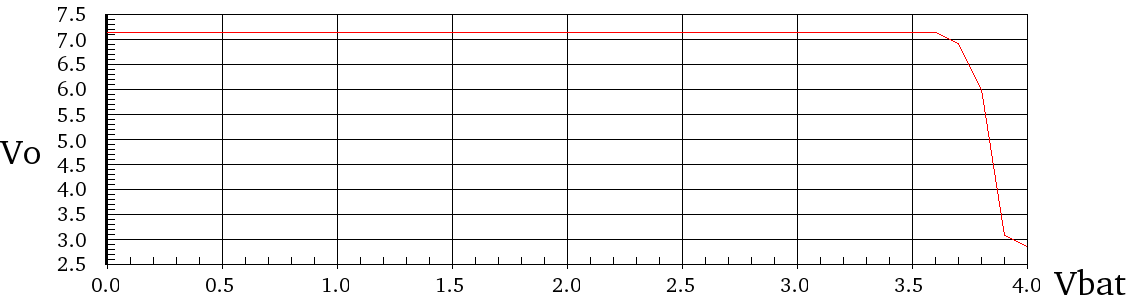
\includegraphics[width=\textwidth]{Imagenes/Bitmap/Capitulo4/simulation1}}  

\subfloat[Current flowing through the battery depending on the its voltage.]{\label{fig:cap4:simulation2}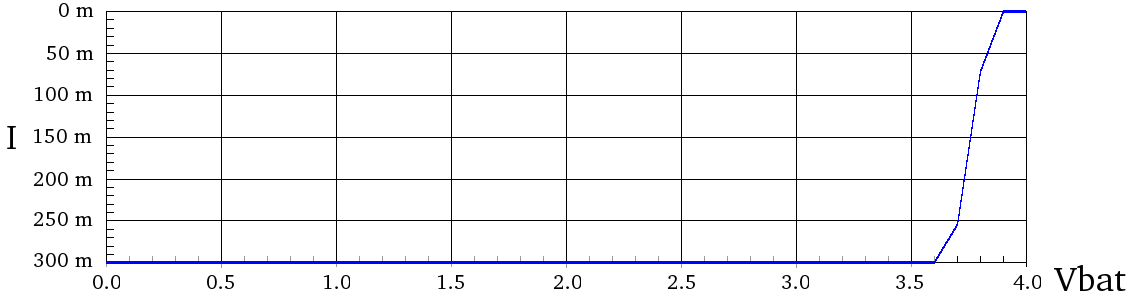
\includegraphics[width=\textwidth]{Imagenes/Bitmap/Capitulo4/simulation2}}
       
\caption{chargerSHIELD simulation results.}
\label{fig:cap4:simulation}
\end{figure}

% Variable local para emacs, para  que encuentre el fichero maestro de
% compilaci�n y funcionen mejor algunas teclas r�pidas de AucTeX
%%%
%%% Local Variables:
%%% mode: latex
%%% TeX-master: "../Tesis.tex"
%%% End:
